% Chapter Template

\chapter{Design and Development} % Main chapter title

\label{DesignAndDevelopment} % Change X to a consecutive number; for referencing this chapter elsewhere, use \ref{ChapterX}

\lhead{Chapter \ref{DesignAndDevelopment}. \emph{Design and Development}} % Change X to a consecutive number; this is for the header on each page - perhaps a shortened title

%----------------------------------------------------------------------------------------
%	SECTION 1
%----------------------------------------------------------------------------------------

Describe the process of development,
and which parts of \theartefact\ which were developed during the different stages of development.
We are then going to give a high level overview of the system before we present each part.

\section{The different phases of development}
We will now describe the different phases of development.
This will outline the main sequence in which work on \theartefact\ was done.
This overview of the iterations will explain when the initial development of
the different part were to give an short explanation of the development process.

\subsection{Iteration 1}
The first iteration started with a technical peak exploring different tools and frameworks for development with javascript.
We wanted to find tools that could reduce development time by reducing the amount of repetitive work done in the project.

It was decided that we were going to use bootstrap\footnote{\url{http://twitter.github.io/bootstrap/}} as a grid system
for the webpage.
Using a standard grid system makes it easier to create a webpage that looks OK,
and reduces the amount of time needed to set up a scaffold.
Since the visual aspect of the webpage was not an important aspect of the work a simple grid system like bootstrap
eased the development burden.

We also decided to use SASS\footnote{\url{http://sass-lang.com}} to write our stylesheets.
The syntax is similar to that of CSS.
We decided to use this instead of CSS since it contained variables,
making it posible to make global changes while only modifying one line in the stylesheet.
SASS compiles to standard CSS.

JavascriptSince javascript lacks a good IDE we wanted to have some tool that would check our code to make sure that the
code was consistent and that the syntax was correct.
We decided to use jslint\footnote{\url{http://www.jslint.com}} to validate our code.
Using a linter eases development as it enforces a particular coding standard for the project.
The way the project was set up, we couldn't build the project without it passing the linting test.

Since the project depended on compiling the stylesheet and linting the code we decided to use grunt.js\footnote{\url{http://gruntjs.com}}
to automate this process.
Grunt.js is a task manager that can run certain tasks when specified events are triggered.
We set the project up so that each time a javascript or SASS file was saved we compiled the SASS document,
and concatenated the public javascript files.
Concatenating the javascript files meant that we didn't have to update the HTML when we created or deleted a new
javascript file, since we only needed to include that one file.

We had decided to use Node.js as the development platform of the project.
Setting up a basic server in node.js can be done in a single line of code,
but requires a lot of low level handeling of requests and responses
including parsing request url to find the correct handler.
We decided to instead go for express\footnote{\url{http://expressjs.com}},
a web app framework which simplifies routing requests to the correct handler and handeling static files.
It was also decided to use the jade\footnote{\url{http://jade-lang.com}}
templating language to generate the HTML that was used on the website.
Using a templating language made the distinction between structure and content clearer,
and enabled reuse of structure and content between different versions of the website during development.

Our technological peak also included geting to know the DOM, the API used for manipulating HTML documents.
The problem we tried to solve during this technical peak was how to find minimal legal ranges.
We knew we were going to have to add separate tags to add the metadata we create,
and that we were going to let users select which portions of the text that carried the semantic content.
Since the user selection might not be a legal HTML range we worked on an algorithm to find the smallest range that
was both a legal range, and which contained the whole of the selected text.


\subsection{Iteration 2}
The next step consisted of actually generating metadata tags with the correct RDFa syntax which enclosed the user selection.
One of the tasks was giving each selected section a unique id so that they could be referenced externaly,
we also wanted this id to carry some information about the content of the tag.
At this stage we had not yet started with development of the mapping so the tags contained mock data.

In this iteration we also started work with generating the hypernym chains we needed to find mappings.
We initially tried to use an existing triple store and query the information with SPARQL.
The triple store used an early version of SPARQL which did not allow recursive queries.
Since we needed to find the transitive closure of the hypernym relation,
using this source would require multiple sequencial queries and would take to long to be tenable.
Javascript does not have a mature library for querying the WordNet database, so we did not have a native solution.
Our solution was instead to use perl to write a script which could query a local WordNet instance.
This again required a technical peak to learn the basics of the perl programming language but gave a satisfying solution.

We also used this iteration to find WordNet mapping files and convert them to a format more suitable for our system.
We had a mapping file between WordNet and SUMO in the WordNet database format,
and one between WordNet and schema.org in RDF.
Both of these files were translated into javascript objects.

\subsection{Iteration 3}
In the third iteration we implemented the actual mapping algorithms that we wanted to try out.
We implemented one that starts with looking at all the hypernyms of the synset,
and one that looks alternately at hypernyms and siblings.

This was also the iteration where we created a mechanism for fetching HTML from other websites so that they could be
marked up using \theartefact.

\subsection{Iteration 4}
In the fourth iteration we made the export module.
This module would take the webpage that the user had imported into the system and create a new HTML document.
This document would be stored in our database, and would be accessible for the user through a URL which we provided when the page was exported.

Adding properties to entities was also developed during this stage.
This was only implemented for schema.org properties,
both to keep the number of properties at a managable level,
and because extracting all the allowed properties for all SUMO classes would be a difficult task.

In this iteration we also added the ability to add author information.
This is not closely tied to the problem of translating natural language to formal ontologies,
but it is tied to allowing users to add metadata in a simple way without knowing about the formal underpinnings.

\subsection{Iteration 5}
The last iteration consisted of testing and refactoring the system.
We wrote some test scripts that would run the best fit algorithms we had created over a set of synsets,
and print out the resulting mappings along with information about whether the algorithms gave corresponding results,
and the measure of quality of the mapping.
The results of these tests will be discussed further in section \ref{ComparingAlgorithms}.

\subsection{Overview completed system}
The artefact was divided into several modules which function independently of each other.
The modules were loosely coupled so that each module could be changed or modified without affecting the other modules.
The modules that were created were:
\begin{itemize}
	\item The web front end
	\item A module that fetched and processed the HTML from the sites that the user wanted to mark up
	\item A module for fetching possible disambiguating terms from lexitags
	\item A module for finding the best fit mappings for SUMO and schema.org
	\item A module for finding the best fit mappings from DBPedia to schema.org
	\item A module that puts the document back in its initial state and saves it to a persisten storage
\end{itemize}

\section{Designing the algorithms}
We will now describe the two algorithms that were developed to find mappings between the WordNet synsets and the ontologies.
We use two axes for navigating the WordNet graph, the hypernyms and the hyponyms.
As described in \ref{WordNet}, a hypernyme can be described as category words into which more specialized words fall.
Hyponyme is the inverse relation, where a hyponyme is a word which can be generalized into some more general category.
For simplicity we will also use one additional term.
We will use \emph{sibling} to refere to words which are hyponymes of a words hypernyme.
An example( see figure \ref{Hyponyme}, page \pageref{Hyponyme})
would be that \{dog\} has the hypernyme \{domestic\_animal\}, which again have the hyponyme \{cat\},
\{cat\} would then be considered a sibling term of \{dog\}.


Our hopes for this mapping tree is that in the cases where there is no direct mapping from the synset to a term in the
ontologies we are mapping to, we can always preserve the semantics of the synset by using one of the synsets ancestors.
For the siblings we hope that if we find a mapping,
then the parent term of the term we have mapped to in the ontology will correspond to the meaning of the synset.
Both these propositions will be tested as a part of the work with the thesis.

The algorithms define different orders of looking at the synsets

\subsection{Generating the search tree}
The first step of the algorithm is the same for both algorithms.
A search tree is generated using a perl script
\footnote{Perl script found at \url{https://raw.github.com/EivindEE/SemTag/master/scripts/parents.pl}.}.

\begin{figure}[ht]
	\begin{center}
		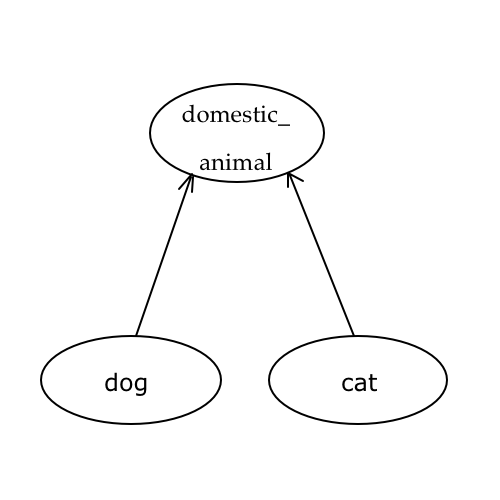
\includegraphics[width=0.60\textwidth]{Hyponyme_own.png}
		\caption{The hyponyme relation, modified from \protect \citet{Miller1990}}
		\label{Hyponyme}
	\end{center}
\end{figure}



\subsection{The sibling first algorithm}
The sibling first algorithm traverses the search tree by first looking if there is a direct mapping from the base synset to the ontologies.
If a direct mapping is not found, it will look at the hypernyms and see if it has a mapping.
After looking at the hypernyms it will look at the sibling senses.
It will then go on to look at the hypernyms of the hypernyms, and then their sibling states.
It will continue to follow the hypernym chain upwards until there are no more hypernyms, or a mappings has been found.

\subsection{The ancestors first algorithm}
The ancestor first algorithm will follow the hypernym chain upwards looking for mappings.
The algorithm is written to follow the hypernym chain again, looking at the sibling senses, if no mapping is found.
But since every WordNet noun is a hyponyme of {entity}, which should map to the most general object in an ontology,
it will likely never be touched.



\section{Interaction method}
\label{Interaction}
When we first faced the problem of how to let users interact with the web app we thought that using the highlighting or
selection of text to be the most intuitive approach.
We also believed that this would be the simplest interaction method to implement.
The simple case of taking selected text and displaying it in the console can be implemented as in listing \ref{DOMSelection}.

\begin{lstlisting}[caption={Logging selected text}, label=DOMSelection]
	var logSelection = function () {
		console.log(window.getSelection().getRangeAt(0).toString());
	};
	document.addEventListener('mouseup', logSelection);
\end{lstlisting}

The "mouseup" event is triggered every time the user has pressed and then released the mouse pointer on the website.
This event is not available on mobile and tablet type browsers,
but adding listeners for corresponding events should not be difficult if we later see the need for this.

In the web app the selected text is sent to the web server to find possible disambiguations for the text.
The lexitags service that we use for disambiguation now is targeted towards disambiguating single words.
It does handle some composite terms and some proper nouns, but this is outside the normal use case.
The lexitags service is designed to disambiguate single tags, not large paragraphs of text.
To accommodate this we do a simple check for the length of the text string.
If the length of the string is more than the longest allowed length,
the query is instead replaced with a shorter query indicating that the selection is of a larger section of text.

The response from the server is a JSON string containing the terms that were found to be possible senses of the selected text.
Each of these senses have an explanation property which gives a short textual description of the meaning of the sense.
These senses are displayed as a list on the web site.
The senses that are returned come from different sources.
They can come either from WordNet and take the form of WordNet synsets, or they can be resources from DBPedia.
Both of these can be used to generate mappings,
but the most interesting mapping for this thesis lies in generating mappings from WordNet so the synsets are given preference in the list.
DBPedia does not have a standardized way of finding the super type of a resource,
so if the resource does not have a schema.org mapping it is difficult to find generalizations that do.
Lexitags also returns the top level resources from schema.org as shown in figure \ref{TopLevelSchemaOrg}(page \pageref{TopLevelSchemaOrg}).
These are sorted to the bottom of the list as these are fallbacks for when none of the of the terms suggested for
the word turn out to be reasonable suggestions for the selected text.

\subsection{Adding types}

To select one of the terms from the list as the meaning of the selected text the user clicks the sense in the list see in
figure \ref{SidebarMeanings}.
\fig{SidebarMeanings}{The list of posible interpretations of "discoveries"} % IMAGE OF LIST OF INTERPRETATIONS
When a sense is clicked it is sent to the server to be mapped.
The servers uses the best fit algorithm described in \ref{BestFitMapping}(page \pageref{BestFitMapping}) to find the ontology references
that fits the sense best and attaches these references to the selection using RDFa.
The algorithm used to attach the metadata to the selection can handle an arbitrary amount of namespaces and references.
If there is duplication of references these will be dropped.

When the metadata element is created,
the schema.org type is sent back to the server to get a list of the possible properties of that type.
On the server we use a JSON representation of the schema.org ontology to find the properties that a type can have.
The representation we use was retrieved from \url{http://schema.rdfs.org} which is a support site that tries to
promote linked data.
For each of the types in schema.org the JSON file provides the properties specific to that type,
and all the properties it has inherited from its super types.
We combine the information about which properties a type can have with a short description of what the property represents,
and information about the range of the property, that is the range of values that are valid values of the property.
The resulting JSON object is then returned to the website.
These properties are then added to the metadata element as separate elements,
with the description and range stored as data attributes of the element.

\subsection{Adding properties}

Users can click text that has been tagged with metadata.
This triggers a popover view which displays the properties that the element can have,
and which types of values are allowed for each property as shown in figure \ref{PropertiesFull}.
\fig{PropertiesFull}{{The properties popover for schema:Event}} % IMAGE OF PROPERTY SELECTION BOX
If the property allows other schema.org types as their value we do a scan of the content of the website to check if
there are elements of the correct type on the page.
Elements of the correct type that are found are put in a combo box and can be selected as values for the property.
In all cases the user is presented with the option of writing the value of the property in an input field.
If the property already has a value it will be displayed in the input field when the popover is displayed.

%\fig{Sidebar}{The information tab of the sidebar},

\section{Maintaining the well-formedness of the document}
One of the difficult aspects of adding the metadata to the selections was making sure that the HTML was well-formed
after the metadata was inserted.

Special care needs to be taken with the ranges of the selection.
Since we need to insert the metadata into tags we can't just use the user range without some checks.
If we consider the simple case:

\texttt{<p>some text \hl{in a p</p> <p>` pluss some} other text </p>}

If we simply inserted a tag we would get invalid HTML since we would have overlapping elements.

\texttt{<p>`some text <tag> in a p</p> <p> pluss some </tag>  other text </p>}

To get a well formed HTML document we need to either close and open the HTML tags

\texttt{<p>some text </p><tag><p> in a p</p> <p> pluss some </p></tag><p>  other text </p>}

Solving the problem in this manner would change the structure and rendering of the webpage,
as we would create new block elements.
This is not a tenable solution as we want to leave the page looking the same as we found it.
Our solution would instead expand the range of the selection so that it covered a larger part of the document:

\texttt{<tag><p>some text in a p</p> <p> pluss some other text </p></tag>}

The interaction method consists of letting the user make arbitrary selections and then adding metadata to the selection.
This could easily lead to overlapping elements in the HTML as shown above.
To avoid this malformed HTML we check the range of the selected text and see if surrounding it with a tag
containing metadata would result in a well-formed document, and modify the range if needed.
If the start and end of the selection are in the same element then adding metadata is safe.
If that is not the case we find the smallest change we need to make to the scope of the range to make it safe.
There are two general cases her, when either the start or the end of the range is in a descendant element of the other,
and when both start and end are descendants of a common element but not of each other.

In the first case we need to find out which element is the descendant of which.
We do that by following the ancestor links of each element.
When we find that either the start or end element has the other as an ancestor we use the ancestor which is the direct
child of the other element and place the start or end tag right before or after that tag, depending on which element
descended from which.

When the elements are not descendants of each other we know that they must be descendants of some other element.
If nothing else they must both be descendants of the root element.
We use a similar approach for this case as we do for the fist,
but instead of finding the ancestor which is the direct child of the other node we find the one which is a child of the
closest common node.
We then surround these elements with the metadata tag.
This metadata element is styled with a distinct color to let the user know that the text is tagged.

\section{Importing webpages}
One of the issues that came up early was how to import and display the websites that the user wanted to add metadata to.
Early attempts tried using the iframe\footnote{http://www.w3.org/TR/html5/embedded-content-0.html\#the-iframe-element}
element of \nom{HTML}{HyperText Markup Language}.
Embedding the target website in an iframe was the first try as it would allow the page to display in the same maner
as it does when accessed directly.
Using the iframe element in this maner would however constitute cross-domain communication and is not allowed.
The solution that is used in the system now uses a module on the server to fetch the HTML of the document the user wants to enrich.
The HTML that is imported is now appended to a content element in the webapp.
We attach the javascript events used in the webapp to this element,
to keep the interaction confined to the content the user is meant to tag.
We also use the id of this tag to tell if a certain element is a part of the user content section by checking if it is
the child of the element.

The user writes the URL of the webpage into an input field on the top of the webapp as shown in figure \ref{MadameHeader}.
\fig{MadameHeader}{The header of the \theartefact\ webapp} % IMAGE OF THE HEADER OF MADAME
The server will fetch the document stored at that location.
We created a proxy to get the html from other websites.
The proxy would take a URL and get the resource located there.
If the resource is not of the right type i.e. not a HTML document with a body element,
the proxy would return an error.
When the resource has been downloaded the content of the body element of the document is parsed to comment out code that
could be harmful, that could make the page display incorrectly, or that could disrupt the way the webapp functions.
The parts of the page that we comment out are the script, iframe and comment elements.
The script elements could disrupt the way the web app works, either by overwriting the behavior of functions,
or otherwise alter the behavior of the web app.
In addition the script elements are not visible on the page so interacting with them would be hard.
Removing them was also convenient durring development.
The scripts in the tags would often rely on variables or functions that should have been loaded elsewhere,
and they would cluttre the console making it more difficult to find the relevant information.
Iframes were excluded since they could make the web app appear to be inconsistent.
The iframes look like a part of the page,
but it would not be possible to alter their content since the HTML belongs to a different document.
The difference between the document and the iframe would be invisible to the user,
so it was decided that it would be better to remove the element all together.
The comment elements were removed to make sure that the page would display as it should.
Since we use comments to remove iframes and scripts, and since these elements could them selves contain comments,
the content of the comments would sometimes be displayed as text elements on the page.

\Theartefact\ is only designed to add metadata to the body element of the document,
so the page is split into body and head parts before it is returned to the webapp.
The document is returned as a JSON string with one property containing the processed body,
and one containing the content of the head.


\section{Generating mapping files}
An important part of the early work was to generate files that the tool could use to find mappings from WordNet synsets
into the ontologies which were used.
The ontologies that were chosen for the project, SUMO  and schema.org, already had these kinds of mapping files.
The mapping files were however in different formats and in formats that were unsuitable for use in a javascript based application.
The format we wanted was one that gave up the option to ask if there was a mapping for a given WordNet synset,
in other words what we wanted was a dictionary.
Javascript objects are themselves dictionaries, making it natural to choose to them as the representation.
The structure of the objects is very simple,
the synsets are used as the keys to entities in the target ontologies as seen in listing \ref{wn2schemaMapping}.

\begin{lstlisting}[label=wn2schemaMapping, caption={Excerpt from the \href{https://github.com/EivindEE/Madame/blob/master/mappings/wn2schema.js}{wn2schema.js} mapping file}]
exports.mapping = {
	"abstraction#n#6": "Intangible",
	"accounting_firm#n#1": "AccountingService",
	"address#n#6": "PostalAddress",
	// The rest of the mappings
	"work_unit#n#1": "Energy"
};
\end{lstlisting}

Since we use javascript objects to represent the mappings,
querying a mapping object to check if it contains a mapping for a certain synset would then just consist of checking if
the object has a property with the given name as in listing \ref{LabelExists}.
\begin{lstlisting}[label=LabelExists,caption=Testing if a mapping exists]
	if (mapping['synset-to-check']) {
		// it contains a mapping
	} else {
		// it does not contain a mapping
	}
\end{lstlisting}

The mapping files were to large to translate to javascript objects by hand, with the SUMO mapping file alone
covering more than 82.000 mappings, so we used regular expressions to modify the files globaly.
The schema.org mapping file\footnote{\url{https://github.com/mhausenblas/schema-org-rdf}}
that was used as the basis for the wn2schema mapping file is written in \nom{RDF/XML}{An XML representation of RDF}.
The first step in creating the mapping file was to remove the parts of the file that were irrelevant to the problem at hand.
The original file contains triples describing schema.org properties,
the schema.org entities and the hierarchal ordering of entities.
This information is handled at other places in the tool we are creating and could be safely removed.
Only the elements mapping synsets to schema.org terms were kept, and all other information except the names were removed.
At this point the XML tags were stripped so only the synset reference and the schema type remained.
Since we now had the correct elements in the correct place we needed only to surround them with the correct quotation
marks, separate them with a colon and add a comma at the end to separate it from the next property.

The SUMO\footnote{\url{http://sigmakee.cvs.sourceforge.net/sigmakee/KBs/WordNetMappings/}} mapping followed a similar pattern,
but the original format was different as it used the WordNet database format.
We used the WordNetMappings30-noun file as our basis so for this mapping we did not have to remove non noun phrases.
The fact that each line in the file corresponded to a line in the mapping file made the process of translation easier,
there was however one caveat in that the file used the offset to identify the synset,
instead of the word\#category\#number format which we use for the other mapping file.
We put some work into finding a way of substituting the offset for the synset id,
but found that it was simpler to find the offset for the synsets that were queried.
Unifying the way the mapping object properties are named is one of the things that can simplify
the generalization of the process at a later stage.



\section{Building the hypernym chain}
\label{BuildingTheHypernymChain}
Many synsets that the users will select as representing the concepts in the web app will be more specific than
the ones used in ontologies \theartefact\ maps to.
This means that the tool needs some way of generalizing the synsets.
This thesis examines two approaches to finding mappings from the synset to the ontologies.
One approach is to use the hypernym chain,
a term used in \citet{Veres2011} to describe the list of all the hypernyms of a synset.
The other approach examined is to use the sibling senses of the synset and the synsets in the hypernym chain.

Javascript does not have a library for 	querying the WordNet database,
so this part of the project needed to be coded in another language.
Had there been a javascript library for querying WordNet,
it would be natural to generate the hypernym chain while searching for the mappings from the synset to the ontologies.
Having to use a different programming language and calling it outside the program,
it is easier and more efficient to split the process.
The system will first generate the entire hypernym chain and add the siblings of all of the hypernyms,
and then examine the hypernym chain to find the best mappings.
This section will describe the first part of this process, generating the hypernym chain.

The system uses a perl script\footnote{\url{https://github.com/EivindEE/Madame/blob/master/scripts/parents.pl}} to generate the hypernym chains.
The script is called by using the node
child\_process.exec\footnote{\url{http://nodejs.org/api/child\_process.html\#child\_process\_child\_process\_exec\_command\_options\_callback}}
function, which calls a command line utility and uses the output stream as the input to the callback function.

The structure of WordNet as a whole can be described as a directed graph, as shown in figure \ref{WordNetGraph}.
The graph must also be acyclical since the hypernym relation is asymmetric as mentioned in section \ref{Hypernymy}.
\fig{WordNetGraph}{Part of the WordNet graph}
Each synset can be described as a node in this graph, with a directed edge connected to its direct hypernym.
For each node in the graph it is also true that following one of the directed edges will lead to the synset entity,
which is the most general concept in WordNet.

The hypernym chain we generate is a list of objects.
The objects contain the hypernym itself, its offset in WordNet, and a list of all its siblings.
Each sibling is stored as an object containing the synset, and its offset.
An example of how the hypernym chain is represented as JSON can be seen in listing \ref{PerlHypernymChain}.

\begin{lstlisting}[float=t, label=PerlHypernymChain, caption={Excerpt from the hypernym chain for student\#n\#1}]
{
	"chain": [
		{
			"synset": "enrollee#n#1",
			"siblings": [ { "synset" : "self#n#2", "offset" : "09604981" ...},
			],
			"offset": "10059162"
		},
		{
			"synset": "person#n#1",
			"siblings": [],
			"offset": "00007846"
		}
	],
	"synset": "student#n#1",
	"siblings": [],
	"offset": "10665698"
}
\end{lstlisting}

Generating the hypernym chain is done in two steps.
The first step is to create a list of all the hypernyms,
while the second is to add all the siblings.
To generate the list of hypernyms, the script does a breadth first traversal of the graph as described in listing \ref{HypernymChainCode}.
For the graph in figure \ref{WordNetGraph} the algorithm would add \{living thing\},
and \{causal agent\} before adding \{physical entity\} and \{entity\} to the list.
If a synset is encountered multiple times, it is ignored in subsequent encounters.
The hypernyms are added to the end of the list when they are found.
This means that the synsets that are at the start of the list,
are the ones that are at the closest level of abstraction to the synset for which we build the chain.

\begin{lstlisting}[float=t, language=perl, label=HypernymChainCode, caption={Excerpt from the hypernym chain perl script}]
my @hypernym = hypernym($synset);
my @hypernyms;
while ( @hypernym){
	my $hypernym = shift @hypernym;
	push(@hypernym, hypernym($hypernym));
	push(@hypernyms, $hypernym);
}

my @hypernyms_with_siblings;
push(@hypernyms_with_siblings, {"synset" => $_ , "offset" => $wn->offset($_) ,"siblings" => [siblings($_)]}) for @hypernyms;

my %result_map = ("chain" => [uniq(@hypernyms_with_siblings)], "synset" => $synset, "offset"=> $wn->offset($synset), "siblings" => [siblings($synset)]);
my $json = JSON->new->utf8->pretty->encode(\%result_map);
print $json;

sub hypernym {
	my @hypernym = $wn->querySense($_[0], "hype");
	if ($#hypernym > 0) {
		return ();
	}
	return @hypernym;
}
sub siblings {
	my $synset = $_[0];
	my @hypernym = hypernym($synset); # Find hypernym of synset
	my @siblings;
	my @sibling_and_offset;
	push(@siblings, $wn->querySense($_, "hypo")) for @hypernym;
	for my $sibling (@siblings) {
		push (@sibling_and_offset, {"synset" => $sibling, "offset" => $wn->offset($sibling)});
	}
	return @sibling_and_offset;
}
\end{lstlisting}


After the list of hypernyms has been created it is iterated over to add the siblings of each of the hypernyms.
For each synset in the hypernym chain the script will find the synsets hypernym,
and then find all the hyponyms of the hypernym.
These sibling senses are then put in a list along with the synset.

\subsection{Problems with multiple hypernyms}
When starting work on the best fit algorithms it was discovered that some hypernyms lead to incorrect mappings.
The problem was noticed when mapping the synset quotation\#noun\#2,
described as "a short note recognizing a source of information or of a quoted passage",
which was mapped to the schema.org term MusicRecording.
This error was caused by the fact that the hypernym chain of quotation\#noun\#2 contains
section\#n\#1 which is a hyponym of both music\#n\#1 and writing\#n\#2, shown in figure \ref{IncorrectHypernyms}.

\fig{IncorrectHypernyms}{The start of the hypernym chain of quotation\#noun\#2}

The synset music\#n\#1 is described as "an artistic form of auditory communication incorporating instrumental or vocal tones in a structured and continuous manner".
The fact that quotation\#noun\#2 is a hyponym of music\#n\#1 violates the rules for hypernymy discussed in \ref{Hypernymy}.
Hypernyms are supposed to be generalizations of its hyponyms,
and they should be in a "is a" relationship to each other.
A native user of english would not say that a quotation is a type of music in the senses of the words are described above.
This error has been reported to the maintainers of WordNet and will be fixed in the next public release( C. Fellbaum, personal communication, May 1).

The main problem this caused was that it made it unclear if both hypernyms would maintain the meaning of a synset,
when the synset had more than one hypernym.
It's not possible to choose a strategy where one only picks one of the hypernyms since the system has no way of
knowing which of the hypernyms to choose.

The system now handles cases where a synset has multiple hypernyms by aborting the generation of the hypernym chain,
and only using the hypernyms found up to that point.
This cutoff can be seen in the hypernym subroutine in the perl script in listing \ref{HypernymChainCode}.
This is not an optimal solution as it discards a lot of synsets which would give good mappings.
It was however chosen to avoid getting extra incorrect mappings when testing the system.
The solution chosen was also simpler to implement than check against hypernyms that were found to be wrong,
and a more sophisticated solution to choosing hypernyms was decided to be outside of the scope of the research problem.

\section{Best fit mapping}
\label{BestFitMapping}
The first step in finding the best mappings for a given synset is finding which mappings exist.
This is done by traversing the hypernym chain and checking for each synset in the chain if it has a mapping to
one of the ontologies we are mapping to.
When the hypernym chain has been modified to include mappings to the different ontologies we can use the different
best fit algorithms and use their traversal of the chain to find which of these mappings that are the best according to
the algorithms.
Both algorithms will start by looking at the synset itself.
We use the direct mappings of the synset should they exist as we have no reason to believe that we can do better than a
direct mapping.
Given that there are ontologies that have not been mapped to we use the best fit algorithms to find the missing mappings.

\subsection{Hypernyms first}
The hypernyms first algorithm traverses the hypernym chain by first looking at the direkt hypernym of the synset for mappings.
It will then follow the hypernym chain upwards as long as no mappings has been found.
This means that,
except in cases where the generation of the hypernym chain is aborted because of multiple hypernyms such as mentioned in section \ref{BuildingTheHypernymChain},
the algorithm will allways map to the most general type of the corresponding ontologies instead of looking at the siblings.
%%% Include in discusion section on other traversals that could give better
\fig{HypernymChain}{{A hypernym chain with siblings}}
Looking at figure \ref{HypernymChain}, the hypernyms first algorithm would follow the links upwards to the top.
If there are no mappings in the hypernym chain the algorithm will start to look at the siblings,
and them looking at them in the same order as the hypernyms.
It will start looking at the siblings of the synset and see if any of them have a mapping.
As long as there are ontologies without mappings it will then follow the hypernym chain upwards again,
this time looking at the siblings of the hypernyms.
If the mapping we find belongs to a sibling of the synset or one of its hypernyms we use the super type of the mapped
type as the type that is mapped to.

\subsection{Hypernym then siblings}
The hypernym first algorithm is conservative.
Since hypernymy is a "is a type of" relationship there is little chance that the resulting mappings can be mistaken.
It does however move quite quickly up the hypernym chain leading to mappings to types that are at higher level
of abstraction than the synset.
Our other try at creating an algorithm tries to stay at a closer level of abstraction by looking at the siblings earlier
in the traversal.

The algorithm still starts by looking at the hypernym.
Since we use the super type of the mapped type when looking at sibling synsets,
it is reasonable to assume that a mapping from the hypernym would we at an equal level of abstraction as the
super type of a sibling mapping.
The algorithm diverges from the hypernyms first by looking at the siblings of the synset after looking at the hypernym.
It will then follow the same procedure up the chain, first looking at each synsets hypernym,
then looking at its siblings before moving up the chain and repeating the process.
Looking again at figure \ref{HypernymChain} we would at each node first look at the node above,
and then at the nodes to the right, before moving one node up the tree.
The maner in which the algorithm choses which sibling to map to is at the moment fairly naïve.
The algorithm will use the first match it finds,
meaning that if two or more siblings have mappings to an ontology the first one found by the algorithm will be used.
As shown in listing \ref{HypernymChainCode} the order of the siblings in the JSON is the same as the order that they
are given by querying the WordNet database.
For our purposes this is equal to using an unordered list since we don't know and can't predict the order.
The for the algorithm we developed for this too we assume  that we have no reason to prefere one mapping over another,
since we at this point don't know the meaning of the synset.
Further refinement is likely posible of this assumption does not hold.

\section{Exporting the document}
To export a page after adding metadata the user clicks on the export tab in the sidebar and on the export button.
This will provide the user with a link the the website with the metadata added as shown in figure \ref{SidebarExported}.
\fig{SidebarExported}{The export tab after exporting the current page} % IMAGE OF EXPORT PANE
The exported site is parsed to put the javascript and iframes back in so that the website look the same as it did
before it was imported into \theartefact.
On the export pane we also give the user the option to add a google plus id to an authorship tag on the page.
This is treated as a separate task as it pertains not to the content of the page, but to the page it self.
It is also not a part of the schema.org ontology, but is included as it is a natural way to increase the visibility of
the website in search results using metadata.

We use MongoDB\footnote{\url{http://www.mongodb.org}} as a database for storing the webpages after the user has added metadata.
MongoDB is a NoSQL database which uses javascript as its database interaction language.
MongoDB uses a dynamic schema for storing data,
meaning that each document in a collection does not need to have the same structure.
This makes it suitable for projects with a rapid development style since the schema does not have to be
finalized at early stages of development.
The artefact uses mongoose\footnote{\url{https://github.com/learnboost/mongoose}} as a tool for modeling the objects.
Mongoose allows us to abstract a lot of the database logic away and simplifies connecting with the database.
When receiving a document to store the module removes all the extra comments that were added when the document was
imported, and puts the document back in its original state.
We also store the namespaces used in the document and the date on which the document was created.
When the document has been stored successfully the URL of the newly created webpage is returned to the user as shown in
figure \ref{SidebarExported} on page \pageref{SidebarExported}.
If there was an error during the process the user is alerted about what went wrong.
